\chapter{Pruebas y Resultados}

En esta secci�n se muestra una serie de experimentos realizados con la aplicaci\'on desarrollada en este trabajo. Estos resultados sirven para evaluar y determinar los par\'ametros adecuados de los procedimientos y algoritmos aplicados, con el objetivo de mejorar los tiempos de respuesta y lograr una mejor calidad en la planificaci\'on efectuada. A continuaci\'on se describen estas pruebas y sus resultados.

%%%%%%%%%%%%%%%%%%%%%%%%%%%%%%%%%%%%%%%%%%%%%%%%
\section{Ambiente de pruebas} \label{PRUEBAS}

En esta secci\'on se plantea la definici\'on del ambiente donde se realizaron las pruebas, tanto de software como hardware. 

\subsection*{Requerimientos de \textit{Hardware}}

Dado que el sistema propuesto est\'a orientado a ser empleado en sistemas hospitalarios rurales, se utilizaron 4 computadores sin ning\'un requerimiento especial de hardware. Las caracter\'isticas de cada uno de los computadores empleados, se resumen en la Tabla \ref{tab:sistemas}.
\begin{table}[htpb]
\centering
\begin{tabular}{|c|l|l|l|}
\hline
Sistema & Procesador & Memoria RAM & Sistema Operativo\\
\hline
1 & Intel Core Duo 1.83 GHz & 2 Gb & Windows XP \\
2 & AMD Athlon 64 X2 Dual 3600 & 2 Gb & Windows Vista \\
3 & Intel Core 2 Quad 2.40 GHz & 4 Gb & Windows 7 \\
4 & Intel Pentium III 498 MGHz & 512 Mb & Windows XP \\
\hline
\end{tabular}
\caption{Descripci\'on de los computadores utilizados en las pruebas}
\label{tab:sistemas}
\end{table}

En l\'ineas generales, se requiere para una ejecuci\'on m\'inima del sistema, un computador convencional de escritorio con las siguientes caracter\'isticas:
\begin{itemize}
	\item Monitor con soporte de una resoluci\'on mayor o igual a $1024 \times 768$ p\'ixeles
	\item Una tarjeta de video est\'andar con soporte de colores de 32 bits.
	\item Procesador Intel Pentium III (o equivalente) en adelante
	\item Una capacidad de al menos 512 Mb de memoria RAM
	\item Al menos 400 Mb disponibles en disco duro para instalar el sistema
	\item Rat\'on y teclado 
\end{itemize}
 
\subsection*{Requerimientos de \textit{Software}}

Los requerimientos de software son los siguientes:
\begin{itemize}
	\item Sistema Operativo Windows 2000 \cite{REF_MIC} en adelante
	\item Microsoft .NET Framework \cite{REF_NET}, versi\'on 1.1 en adelante
	\item Base de Datos MySQL \cite{REF_MYSQL}, distribuci\'on 5.0 en adelante
\end{itemize}

El sistema fue desarrollado en Microsoft C\# para la interfaz gr\'afica de usuario y varios m\'odulos en C++. Ambas plataformas se comunican empleando librer\'ias de enlace din\'amico (DLL). El ambiente de desarrollo fue Microsoft Visual Studio 2008, utilizando las siguientes librer\'ias adicionales:
\begin{itemize}
	\item Librer\'ia FreeImage \cite{REF_FREE} para el manejo de im\'agenes, versi\'on 1.1
	\item \textit{Driver Connector/Net} \cite{REF_CONNEC} para la comunicaci\'on entre MySQL y C\#, versi\'on 6.3.5
\end{itemize}

Es importante destacar que la aplicaci\'on emplea un tama\~no de ventana de $1024 \times 768$ p\'ixeles y est\'a centrada en la ventana de trabajo. A continuaci\'on se especificar\'an las pruebas realizadas con el sistema CAOS planteado.

%%%%%%%%%%%%%%%%%%%%%%%%%%%%%%%%%%%%%%%%%%%%%%%%
\section{Adquisici\'on de la imagen} \label{adquisicion_image}

Para la adquisici\'on de im\'agenes, se utilizaron las c\'amaras de tres (3) dispositivos m\'oviles y dos (2) c\'amaras digitales. La especificaci\'on de los siguientes se muestran en la Tabla \ref{tab:devices}:
\begin{table}[htp]
\centering
\begin{tabular}{|l|l|c|}
\hline
Descripci\'on&M\'ax. resoluci\'on de Captura&Dimensi\'on m\'ax. de Captura\\
\hline
Tel\'efono Inteligente \# 1 & 4.00 Megap\'ixeles & 2560 $\times$ 1600\\
Tel\'efono Inteligente \# 2& 5.20 Megap\'ixeles & 2560 $\times$ 1920\\
Tel\'efono Celular \# 1 & 3.15 Megap\'ixeles & 2048 $\times$ 1536\\
C\'amara \# 1 & 3.15 Megap\'ixeles & 2048 $\times$ 1536\\
C\'amara \# 2 & 8.00 Megap\'ixeles & 3264 $\times$ 2448\\
\hline
\end{tabular}
\caption{Descripci\'on de los dispositivos de adquisici\'on empleados}
\label{tab:devices}
\end{table}

Tanto los Tel\'efonos Inteligentes \#1 y \#2 y el Tel\'efono Celular \#1 no contaban con sistema de flash. Las C\'amaras \#1 y \#2 ten\'ian dicho sistema interno. Nuestras pruebas se basaron en tomar las im\'agenes de los diferentes dispositivos mostrados. La captura de la imagen se concentra en la placa colocada sobre el negatoscopio. Los dispositivos de captura no emplearon el sistema de flash para la adquisici\'on ya que el negatoscopio garantizaba el contraste de las placas.

Nuestras pruebas demostraron que para abarcar el \'area completa de una placa sobre el negatoscopio, la imagen debe ser capturada a una distancia de 1 m. $\pm$ 10 cm. del centro de la placa y en direcci\'on opuesta al plano donde yace. En la pr\'actica esta distancia es equivalente a colocarse aproximadamente a un paso hacia atr\'as del negatoscopio en el caso de los negatoscopios de pared \'o port\'atiles. Para el caso del negatoscopio de mesa, la c\'amara debe ubicarse a un metro del centro de la misma tomando en cuenta la inclinaci\'on. Para nuestros experimentos, la mesa ten\'ia una inclinaci\'on de $30$\textdegree.

Para adquirir la fotograf\'ia se emplearon tres (3) tipos de negatoscopio: de pared, port\'atil y de mesa. Los dos primeros con un \'angulo de $90$\textdegree  respecto al suelo, ver Figura \ref{fig:nega1}, y el tercero con $30$\textdegree, ver Figura \ref{fig:nega2}.

\begin{figure}[htb]
  \begin{center} 
 \subfigure[]{\label{fig:nega1}\includegraphics[width=0.20\columnwidth]{images/negatoscopio1.png}} \hspace{2.3cm} 	\subfigure[]{\label{fig:nega2}\includegraphics[width=0.20\columnwidth]{images/negatoscopio2.png}}   \end{center}
  \caption{Ubicaciones de las c\'amaras con respecto a los negatoscopios utilizados para la adquisici\'on de las im\'agenes: (a) con un \'angulo de $90$\textdegree con respecto al suelo y (b) con un \'angulo de $30$\textdegree con respecto al piso}
  \label{fig:nega}
\end{figure}

Al colocarse la c\'amara a una distancia menor  del objetivo, la profundidad de campo de la c\'amara hacia que no se abarcara toda la imagen \'o se viera desenfocada. Al colocarse a una distancia mayor, se deb\'ia realizar el enfoque de la c\'amara adem\'as de que era inevitable capturar parte del fondo de la imagen (e.g. la sala de radiolog\'ia, el consultorio, etc.) lo cual no es deseable.

Bajo el escenario descrito, se adquirieron alrededor de 150 im\'agenes. Cada imagen representa un caso en su vista AP (anteroposterior), y en ocasiones se emplean la vista LAT (lateral). Esta adquisici\'on fue realizada completamente en el Departamento de Traumatolog\'ia del Hospital Universitario de Caracas con placas tomadas a diversos pacientes en el Departamento de Radiolog\'ia de la misma instituci\'on hospitalaria.

%%%%%%%%%%%%%%%%%%%%%%%%%%%%%%%%%%%%%%%%%%%%%%%%
\section{Calibraci\'on de la imagen} \label{calibracioni}

En el Algoritmo de B\'usqueda de Orificios presentado en la Secci\'on \ref{AlgBusqOri1}, se mostraron diversos par\'ametros del algoritmo voraz con el objetivo de conseguir dos orificios que representan a los dejados por una perforadora de papel. Las pruebas efectuadas consistieron en variar los par\'ametros de los umbrales $U, T$ y $E$ del Algoritmo de B\'usqueda de Orificios. El prop\'osito de las pruebas es valorar de forma visual los resultados obtenidos en cuanto a la detecci\'on de los orificios de acuerdo a la calidad de la imagen.

%%%%%%%%%%%%%%%%%%%%%%%%%%%%%%%%%%%%%%%%%%%%%%%%
\subsubsection*{Par\'ametro $U$}

El par\'ametro $U$ indica la diferencia entre el promedio de los p\'ixeles recorridos hacia arriba-abajo ($U_h$) y hacia derecha-izquierda ($U_w$), desde el centro de un posible candidato. Si la diferencia es igual a cero, entonces tiene la misma distancia en ambas direcciones siendo esto un factor ideal. Con las im\'agenes de prueba, este escenario sucedi\'o en solo 1 caso, representando $0.67\%$ del total de las pruebas.

En las im\'agenes de prueba de dimensiones $W \times H$ p\'ixeles, donde $W$ representa el ancho de la imagen y $H$ su altura, se recomienda utilizar los siguientes umbrales:
$$U_w = \frac{W}{100 \times k}$$
$$U_h = \frac{H}{100 \times k}$$
$$U = \frac{U_w \times U_h}{2}$$
para valores de $k = {2,3,4}$. Estos valores representan aproximadamente el valor de $\frac{d}{4}$ donde $d$ indica el di\'ametro de un posible candidato que represente a un c\'irculo. Es decir, se considera aceptable como par\'ametro $U$ hasta $\frac{1}{4}$ del di\'ametro de un c\'irculo.

Es importante destacar que la decisi\'on del valor del umbral $U_w$ y $U_h$ debe ser porcentual con respecto a las dimensiones reales ya que no se conocen a priori las dimensiones de la imagen de entrada. El valor de $U$ debe representar una peque\~na porci\'on en p\'ixeles. Si $U$ es muy grande, entonces el n\'umero de candidatos es mayor y si $U$ es muy peque\~no, el n\'umero de candidatos es menor y posiblemente no se considere a los c\'irculos hechos por la perforadora de papel como candidatos.

%%%%%%%%%%%%%%%%%%%%%%%%%%%%%%%%%%%%%%%%%%%%%%%%
\subsubsection*{Par\'ametro $T$}

El par\'ametro $T$, indica la diferencia entre la longitud de los di\'ametros de un posible candidato en forma de c\'irculo. El valor ideal de esta diferencia, debe ser $0$. En el caso de nuestro algoritmo, la diferencia entre la longitud del di\'ametro vertical $d_1$ con la longitud del di\'ametro horizontal $d_2$ est\'a representado como $\mid d_1 - d_2\mid$.

El valor de $T$ permite discriminar candidatos que sean muy ovalados y filtrar los que sean m\'as redondos. Para nuestro algoritmo se tom\'o el valor de $T = \frac{U}{2}$ con el objetivo de encontrar los candidatos con ``mayor posibilidad'' de ser un c\'irculo. Con este criterio se determina que si $\mid d_1 - d_2\mid \le T$ entonces en esa posici\'on es posible haber conseguido el centro $C_{x,y}$ de un c\'irculo.

Con los valores $pN,pS,pE,pO$, ver Figura \ref{fig:circulo}, es posible determinar si una posici\'on $(x,y)$ es el centro de un candidato a orificio basados en los valores de umbral $U,T$. El valor umbral $U$ es la diferencia permitida entre el alto y el ancho promediado de un candidato. Dicho valor va a permitir descartar candidatos que su eje vertical/horizontal sea muy distinto al eje contrario. Es por ello que la verificaci\'on dentro del Algoritmo \ref{busqueda} se hace como $\frac{pN+pS}{2} - \frac{pO+pE}{2} < U$. El valor umbral $T$ es la diferencia entre la longitud de los di\'ametros de un posible candidato en forma de c\'irculo. El valor ideal de esta diferencia, debe ser $0$. Este valor permite discriminar candidatos que sean muy ovalados y filtrar los que sean m\'as redondos.

%%%%%%%%%%%%%%%%%%%%%%%%%%%%%%%%%%%%%%%%%%%%%%%%
\subsubsection*{Par\'ametro $E$}

El par\'ametro $E$ representa el error m\'aximo permitido para considerar un candidato como c\'irculo. Como se mencion\'o en la Secci\'on \ref{AlgBusqOri2}, se utiliz\'o el valor de $E = 12\%$ para considerar los casos en donde la imagen de entrada no sea de buena calidad. Para nuestras pruebas, valores por encima de $12\%$ permit\'ian aceptar candidatos a c\'irculo cuando en realidad representaban otras formas. Por otro lado, valores por debajo de $12\%$ requer\'ian que los candidatos fuesen muy parecidos a una estructura circular siendo muy estricto en su selecci\'on. 

En la pr\'actica, se obtuvieron resultados correctos en 142 im\'agenes de 150 del total. De las 150 im\'agenes, 8 fueron capturadas por la c\'amara sin haber sido perforadas previamente por la perforadora de papel. Estos casos fueron planificados de la misma forma que los dem\'as pero con una calibraci\'on manual. El algoritmo termina sin seleccionar ning\'un candidato posible dentro de la imagen. De las 142 im\'agenes, en 30 de ellas se detect\'o solamente un orificio y en las restantes ambos. En la Figura \ref{fig:orificios} se muestra la distribuci\'on obtenida.
\begin{figure}[htb]
	\centering
		\includegraphics[width=.6\columnwidth]{images/orificio.png}
	\label{fig:orificios}
	\caption{Gr\'afico que muestra el n\'umero de orificios detectados y su proporci\'on sobre el total de 150 im\'agenes estudiadas}
\end{figure}

El Algoritmo de B\'usqueda de Orificios no detecto ning\'un orificio en las im\'agenes que no fueron perforadas. Esto representa el $5.33\%$ de nuestra muestra. Por otro lado, fue detectado un solo orificio en un $20.00\%$ del total y ambos orificios en un $74.57\%$. Como se mencion\'o en la Secci\'on \ref{AlgBusqOri2}, si se encuentra un solo orificio, el otro puede ser ubicado de forma manual. Se recomiendan los valores de $E$ entre un $10\%$ y $15\%$ de discrepancia. Esta diferencia es de acuerdo a la superposici\'on de una m\'ascara construida din\'amicamente que representa un c\'irculo perfecto con el posible candidato. 

En la Figura \ref{fig:testhole} se muestra un ejemplo de los resultados del Algoritmo de B\'usqueda de Orificios. En la Figura \ref{fig:testhole1} se tiene un extracto de la imagen original captada por el m\'edico radi\'ologo enfocada en los orificios. Se puede observar como el algoritmo encontr\'o los orificios empleando los par\'ametros recomendados para $U$ con $k=3$, $T = \frac{U}{2}$ y $E = 12\%$. La Figura \ref{fig:testhole2} muestra la misma imagen pero con un valor de brillo $B=100$, esto quiere decir que todos los p\'ixeles est\'a en el rango de $[100-255]$. En la Figura \ref{fig:testhole3} se aumento el nivel de brillo a $B=150$ y a\'un sigue detectando los orificios. Finalmente, en la Figura \ref{fig:testhole4} se muestra una imagen con $B=200$ donde los valores de los p\'ixeles se encuentran en el rango $[200-255]$ y el algoritmo solamente detecto un solo orificio.
\begin{figure}[htpb]
  \begin{center} 
  \subfigure[]{\label{fig:testhole1}\includegraphics[width=0.16\columnwidth]{images/holes1.png}} \hspace{0.9cm}
  \subfigure[]{\label{fig:testhole2}\includegraphics[width=0.16\columnwidth]{images/holes2.png}} \hspace{0.9cm}
\subfigure[]{\label{fig:testhole3}\includegraphics[width=0.16\columnwidth]{images/holes3.png}}\hspace{0.9cm}
\subfigure[]{\label{fig:testhole4}\includegraphics[width=0.16\columnwidth]{images/holes4.png}}
  \end{center}
  \caption{Im\'agenes extra\'idas de la misma planificaci\'on con diversos par\'ametros de brillo para estudiar el Algoritmo de B\'usqueda de Orificios. (a) imagen original (b) con valor de brillo $B = 100$ (c) con valor de brillo $B = 150$ (d) con valor de brillo $B = 200$}
  \label{fig:testhole}
\end{figure}

El caso mostrado en la Figura \ref{fig:testhole4}, en la pr\'actica suceder\'ia si hubo una mala adquisici\'on de la placa de Rayos-X por parte del radi\'ologo. En estos casos, se repite nuevamente el examen al paciente \'o el mismo es solicitado por el m\'edico traumat\'ologo tratante. Sin embargo, nuestro algoritmo detect\'o al menos un orificio y ubico bastante cerca el otro orificio.

%%%%%%%%%%%%%%%%%%%%%%%%%%%%%%%%%%%%%%%%%%%%%%%%
\subsection{Deformaci\'on del implante}

Para la deformaci\'on del implante se realizaron diversas pruebas a nivel del algoritmo empleado, las restricciones aplicadas y los resultados visuales obtenidos. A continuaci\'on se describen las pruebas realizadas.

%%%%%%%%%%%%%%%%%%%%%%%%%%%%%%%%%%%%%%%%%%%%%%%%
\subsubsection{Algoritmo de Deformaci\'on}

En el trabajo propuesto por Schaefer et al. \cite{SCHAF06} se menciona un efecto de plegado (llamado \textit{foldback}) producto de la deformaci\'on. Adem\'as, Schaefer et al. \cite{SCHAF06} afirman que este efecto para ciertas deformaciones es aceptable. Para nuestro sistema, dicha deformaci\'on provocar\'ia un efecto no deseado ya que cambiar\'ia las proporciones de los implantes. En la Figura \ref{fig:defor2} se puede observar el efecto de plegado al mover el controlador de un extremo de la Figura \ref{fig:defor1}.

\begin{figure}[htbp]
  \begin{center}
  	\subfigure[]{\label{fig:defor1}\includegraphics[width=0.48\columnwidth]{images/def1.png}} \hspace{0.3cm}
  	\subfigure[]{\label{fig:defor2}\includegraphics[width=0.48\columnwidth]{images/def2.png}}   
  \end{center}
\caption{Malla que representa a un implante (a) sin deformaci\'on y (b) con deformaci\'on de plegado}
\label{fig:defor}
\end{figure}

En nuestra propuesta, al emplear un OBB para encapsular el implante se utiliza el \'angulo de rotaci\'on de la caja envolvente con respecto al eje $X$. Esta rotaci\'on se aplica a cada uno de los controladores del implante. En la Figura \ref{fig:arrows} se observa que al seleccionar con el rat\'on un controlador, se indica al usuario la direcci\'on hacia donde se mover\'a dicho controlador para provocar la deformaci\'on en ese sentido.

\begin{figure}[htb]
  \begin{center} 
  	\subfigure[]{\label{fig:arrows1}\includegraphics[width=0.35\columnwidth]{images/handlerMove1.png}} \hspace{0.6cm}	\subfigure[]{\label{fig:arrows2}\includegraphics[width=0.35\columnwidth]{images/handlerMove2.png}} 
  \end{center}
  \caption{Controladores sobre el implante para el doblado. El doblado siempre es en sentido opuesto al eje mayor del OBB que lo contiene. (a) Controladores sin ser seleccionados. (b) Selecci\'on de un controlador e indicadores de la direcci\'on permitida del doblado}
  \label{fig:arrows}
\end{figure}

%%%%%%%%%%%%%%%%%%%%%%%%%%%%%%%%%%%%%%%%%%%%%%%%
\subsubsection{Funci\'on de peso}

Al aplicar \textit{Moving Least Squares} para la deformaci\'on de im\'agenes, el valor del peso de cada punto $v$ de la imagen con respecto a los controladores es un factor relevante que determina el resultado visual de la deformaci\'on. La ecuaci\'on para el c\'alculo del peso es la Ecuaci\'on \ref{ec:ec1}.

En la Figura \ref{fig:defororiginal} se muestra el implante al cual se le aplic\'o las diversas pruebas de deformaci\'on hechas para este trabajo. La imagen tiene un tama\~no de $500 \times 104$ p\'ixeles. El cuadrado con borde verde representa una subimagen de tama\~no $64 \times 85$ p\'ixeles donde se realiz\'o una ampliaci\'on para observar los detalles resultantes de la deformaci\'on.
\begin{figure}[htb]
	\centering
		\includegraphics[width=.8\columnwidth]{images/defororiginal.png}
	\caption{Imagen con los controladores colocados a lo largo del eje mayor. El recuadro verde indica la subimagen a ampliar para observar m\'as de cerca la deformaci\'on}
	\label{fig:defororiginal}
\end{figure}

Se realizaron diversas pruebas variando el valor $\alpha$ de la Ecuaci\'on \ref{ec:ec1}. Dicho valor representa una constante que aumenta o disminuye la tasa de decaimiento de la funci\'on de peso. El objetivo de esta prueba es determinar el resultado visual que se puede obtener al variar dicho valor.

En la Figura \ref{fig:alpha1} se muestra el resultado obtenido con $\alpha=0.5$ y en la Figura \ref{fig:alpha2} con $\alpha=1.0$ (equivalente a $w_i = \frac{1}{|p_i - v|^2}$). En la Figura \ref{fig:alpha3} se tiene $\alpha=1.5$ y finalmente en la Figura \ref{fig:alpha4} se muestra $\alpha=3.5$.
\begin{figure}[htb]
  \begin{center} 
  	\subfigure[]{\label{fig:alpha1}\includegraphics[width=0.24\columnwidth]{images/alpha05.png}}
  	\subfigure[]{\label{fig:alpha2}\includegraphics[width=0.24\columnwidth]{images/alpha10.png}}   
  	\subfigure[]{\label{fig:alpha3}\includegraphics[width=0.24\columnwidth]{images/alpha15.png}}
  	\subfigure[]{\label{fig:alpha4}\includegraphics[width=0.24\columnwidth]{images/alpha35.png}}
  \end{center}
  \caption{Resultados del doblado de una parte del implante variando el valor de $\alpha$, (a) $\alpha = 0.5$ (b) $\alpha = 1.0$ (c) $\alpha = 1.5$ (d) $\alpha = 3.5$}
  \label{fig:alpha}
\end{figure}

El valor de $w$ indica la proporci\'on en la cual la deformaci\'on afectar\'a a los puntos $v$ con respecto a su distancia a los controladores $p_i$. Mientras un punto $v$ se encuentre m\'as alejado de un punto $p_i$, el punto $v$ se ver\'a menos afectado por la deformaci\'on aplicada sobre $p_i$. 

A medida que el valor de $\alpha$ es menor los p\'ixeles de la imagen son menos afectados por la deformaci\'on. Esto implica que se debe realizar un mayor movimiento de los controladores para lograr una deformaci\'on m\'as realista. En este caso el implante da la sensaci\'on de ser un material con mayor rigidez de la que realmente puede tener, siendo entonces una soluci\'on no muy adecuada. Por otro lado, a medida que se aumenta el valor de $\alpha$ la deformaci\'on se hace m\'as flexible y deforma las propiedades de forma original del implante.

En la Figura \ref{fig:alpha1} se muestra como la deformaci\'on afecta en poca medida al implante y da un efecto visual de redondez con respecto al orificio. La Figura \ref{fig:alpha2}, no ofrece una deformaci\'on suave en la parte del borde del implante adem\'as de deformar ligeramente el orificio, lo cual no sucede en un escenario ideal. Por otra parte, la Figura \ref{fig:alpha3} muestra una deformaci\'on un poco m\'as ajustada a la realidad pero cambia las proporciones en el punto de inflexi\'on del implante, modificando su \'area, lo cual es indeseable. Finalmente, la Figura \ref{fig:alpha4} obtiene un resultado que simula un implante muy r\'igido en cuanto a la deformaci\'on de la forma del mismo, y el orificio se estira mucho con el doblado. Dados estos resultados, lo ideal es conseguir una deformaci\'on como la mostrada en la Figura \ref{fig:alpha3} pero sin mucho cambio en el punto de inflexi\'on y menos impacto en la fuerza de la deformaci\'on (cantidad de p\'ixeles que debe mover el controlador para deformar).

Para obtener unos mejores resultados, se probaron otras funciones para determinar la distancia entre los p\'ixeles $v$ y los controladores $p_i$. Una de las funciones empleadas fue la inversa de la distancia de Chebyshev \cite{WEB99} que viene dada por:
\begin{equation}
\label{ec:chebyshev}
	D_{Chevyshev}(a,b) = max_i^n(\mid a_i - b_i \mid)
\end{equation}

\noindent
donde $a_i$ y $b_i$ son dos puntos que representan a $v$ y $p_i$ respectivamente. Otra funci\'on empleada en los experimentos como funci\'on de peso, fue la inversa de la distancia de Minkowski \cite{WEB99} que se expresa como:
\begin{equation}
\label{ec:minkowski}
	D_{Minkowski}(a,b) = (\sum_{i=1}^{n}{\mid a_i - b_i \mid}^k)^{\frac{1}{k}}
\end{equation}

Cabe destacar que cuando $k \rightarrow \infty$ se obtiene la distancia de Chebyshev. En la Figura \ref{fig:func} se muestra el resultado obtenido al aplicar las funciones inversas de las distancias de Chebyshev y de Minkowski. Se puede observar en la Figura \ref{fig:func1} el resultado de la deformaci\'on en la subimagen de estudio, al aplicar Chevyshev. En la Figura \ref{fig:func2}, \ref{fig:func3} y \ref{fig:func4} se observa la deformaci\'on al aplicar Minkowski con $k=0.5; 1.0; 2.5$ respectivamente.

\begin{figure}[htbp]
  \begin{center} 
	\subfigure[]{\label{fig:func1}\includegraphics[width=0.24\columnwidth]{images/chebyshev.png}}
	\subfigure[]{\label{fig:func2}\includegraphics[width=0.24\columnwidth]{images/minkowski05.png}}
	\subfigure[]{\label{fig:func3}\includegraphics[width=0.24\columnwidth]{images/minkowski10.png}}
	\subfigure[]{\label{fig:func4}\includegraphics[width=0.24\columnwidth]{images/minkowski25.png}}
  \end{center}
  \caption{Resultado del doblado de una parte del implante empleando (a) la inversa de la distancia de Chebyshev y la inversa de la distancia de Minkowski con (b) $k = 0.5$ (c) $k = 1.0$ (d) $k = 2.5$}
  \label{fig:func}
\end{figure}

Al aplicar Chebyshev, ver Figura \ref{fig:func1}, el resultado visual no es adecuado ya que se presenta distorsi\'on en los p\'ixeles cercanos al controlador. Para la funci\'on de distancia de Minkowski, la proporci\'on de deformaci\'on aplicada es muy similar, la diferencia radica en la suavidad y continuidad ofrecida en los p\'ixeles cercanos al controlador. En la Figura \ref{fig:func2} se obtiene un resultado aceptable pero se nota en la parte inferior se observa un doblado muy r\'igido, siendo no adecuado para nuestra aplicaci\'on.

Dicha discontinuidad se va tornando m\'as suave a medida que empleamos una valor de $k$ mayor, v\'ease la Figura \ref{fig:func3}. Finalmente, luego de realizar las pruebas con diversos valores de $k$ para Minkowski, se obtiene una deformaci\'on ideal que no deforma los orificios y modela la operaci\'on que se aplica en una sala de operaci\'on para la deformaci\'on de un implante met\'alico. Esto viene representado por el valor de $k=2.5$ como se muestra en la Figura \ref{fig:func4}.

Es importante mencionar que el resultado de la deformaci\'on va a depender tambi\'en de la resoluci\'on de la malla que se utilice para el \textit{Moving Least Squares} como se mencion\'o en la Secci\'on \ref{MLSMalla}. A continuaci\'on se muestran las pruebas realizadas con las dimensiones de la malla.

%%%%%%%%%%%%%%%%%%%%%%%%%%%%%%%%%%%%%%%%%%%%%%%%
\subsubsection{Resoluci\'on de la malla}

La resoluci\'on de la malla define la cantidad de puntos a los cuales ser\'a aplicada la deformaci\'on. Esta resoluci\'on se define como el n\'umero de cuadrados que forman una malla. A un mayor n\'umero de cuadrados, la distancia entre los v\'ertices que lo forman es menor.

Dada una malla con $m \times n$ cuadrados el n\'umero total de v\'ertices de la malla es $m + 1 \times n + 1$. La distancia entre v\'ertice y v\'ertice es constante por ser una malla uniforme. Un v\'ertice $v_{x,y}$ se encuentra a una distancia de $dp$ p\'ixeles de los v\'ertices vecinos $v_{x \pm dp,y}$ y $v_{x,y\pm dp}$. El tiempo de procesamiento es directamente proporcional a la distancia $dp$. En la Figura \ref{fig:dist} se puede observar distintas distancias aplicadas a una imagen de un implante.

\begin{figure}[htb]
  \begin{center} 
	  \subfigure[]{\label{fig:dist1}\includegraphics[width=0.23\columnwidth]{images/distance1.png}} \hspace{0.1cm}
	  \subfigure[]{\label{fig:dist2}\includegraphics[width=0.23\columnwidth]{images/distance3.png}} \hspace{0.1cm}
	  \subfigure[]{\label{fig:dist3}\includegraphics[width=0.23\columnwidth]{images/distance5.png}} \hspace{0.1cm}
	  \subfigure[]{\label{fig:dist4}\includegraphics[width=0.23\columnwidth]{images/distance9.png}}
  \end{center}
  \caption{Diferentes distancias $dp$ entre un par de v\'ertices vecinos (a) $dp = 2$ (b) $dp = 4$ (c) $dp = 6$ (d) $dp = 10$} 
  \label{fig:dist}
\end{figure}

En la Figura \ref{fig:dist1} se muestra una malla con una distancia $dp = 2$ entre par de v\'ertices vecinos, es decir, cada cuadrado tiene un \'area de $4$ p\'ixeles. Se puede deducir que para una resoluci\'on de imagen de $m \times n$ p\'ixeles, se obtendr\'a una mallado de $\frac{m \times n}{dp^2}$ v\'ertices. Entonces, el n\'umero de puntos a los cuales se le aplicar\'a la deformaci\'on se va reduciendo a medida que se aumenta el valor de $dp$ sin afectar la calidad de la imagen resultante. Una distancia $dp = 4$ se emplea en la Figura \ref{fig:dist2}, mostrando una calidad de imagen similar a cuando $dp = 2$.

Al mismo tiempo, se utiliz\'o una distancia $dp = 6$ en la Figura \ref{fig:dist3} donde a nivel visual la calidad es similar a cuando $dp = 2$. Una diferencia a notar es el \textit{aliasing} de las im\'agenes en los bordes. Al tener los cuadrados de la malla de un mayor tama\~no existir\'a un \'area mayor que debe ser cubierta a trav\'es de interpolaci\'on lineal con los v\'ertices que la conforman. 

Para nuestra propuesta se emple\'o un valor de $dp = 5\%$ del lado m\'as largo del implante. Con este valor se obtuvo una calidad visual adecuada luego de aplicar la deformaci\'on. Con valores inferiores a dicho valor, la calidad visual es similar a \'este pero se requiere de mayor c\'alculo computacional. Para valores de $dp > 5\%$, la calidad visual va disminuyendo, provocando la presencia de p\'ixeles indeseados en la imagen. Es importante destacar que el n\'umero de veces que se invoca a la funci\'on de deformaci\'on es directamente proporcional al n\'umero de v\'ertices del mallado. En la Figura \ref{fig:resol} se observa un ejemplo del efecto producido con 2 resoluciones de mallado distintas. En la Figura \ref{fig:resol1} se observa un implante de dimensiones $29 \times 203$ p\'ixeles con una resoluci\'on de mallado de $dp = 10$ que corresponde al $5\%$ de su longitud mayor. En la Figura \ref{fig:resol2} se observa el mismo implante pero con un valor de $dp = 30$ que corresponde al $15\%$ de su longitud mayor. Se puede observar la diferencia a nivel de calidad del implante en ambas resoluciones.
\begin{figure}[htb]
  \begin{center} 
	  \subfigure[]{\label{fig:resol1}\includegraphics[width=0.083\columnwidth]{images/con5.png}} \hspace{1.0cm}
	  \subfigure[]{\label{fig:resol2}\includegraphics[width=0.13\columnwidth]{images/con15.png}}
  \end{center}
  \caption{Ejemplo de un implante colocado sobre una placa de Rayos-X con distintas resoluciones de mallado (a) con $dp = 10$ y (b) con $dp = 30$} 
  \label{fig:resol}
\end{figure}

Al asignar diversos valores a todas las variables de nuestra aplicaci\'on, fue posible determinar un conjunto de par\'ametros ideales para que nuestra soluci\'on se ajuste a la planificaci\'on preoperatoria deseada. El objetivo final es disminuir el tiempo de creaci\'on de dicha planificaci\'on, pero siempre consiguiendo resultados satisfactorios. Para ello, se realizaron pruebas donde se comparan los resultados obtenidos empleando la planificaci\'on convencional con nuestra propuesta. Dichos resultados se muestran a continuaci\'on.

%%%%%%%%%%%%%%%%%%%%%%%%%%%%%%%%%%%%%%%%%%%%%%%%
\subsection{Planificaci\'on convencional vs. Planificaci\'on digital}

Para las pruebas del sistema, se llev\'o a cabo un estudio realizado por el Dr. Carlos S\'anchez del Servicio de Traumatolog\'ia y Ortopedia del Hospital Universitario de Caracas (HUC) \cite{REF_HUC}. Dicho estudio tom\'o lugar a lo largo de un per\'iodo de 4 meses, desde Septiembre a Diciembre 2010. La prueba consisti\'o b\'asicamente en realizar la planificaci\'on preoperatoria a un grupo de pacientes que eran atendidos en el Servicio de Traumatolog\'ia y Ortopedia del HUC.
Para ello, se tomaron en cuenta los siguientes factores asociados al estudio:
\begin{itemize}
	\item Tres m\'edicos realizaron las pruebas en PCs convencionales y port\'atiles cumpliendo con los requisitos m\'inimos descritos en la Secci\'on \ref{PRUEBAS}.
	\item Se planific\'o un total de 20 casos tanto con planificaci\'on digital como convencional donde hub\'o presencia de distintas fracturas de los miembros inferiores. En total, se planific\'o de forma digital 150 casos en un per\'iodo de 7 meses desde Junio a Diciembre 2010. Para los 20 casos se planificaron 12 fracturas de f\'emur y 8 fracturas de tibia. En la Tabla \ref{tab:fractures} se describe detalladamente el estudio.
	\item Por cada planificaci\'on a realizar, un mismo m\'edico realiz\'o tanto la planificaci\'on convencional como la planificaci\'on con nuestra propuesta. Como la planificaci\'on se lleva a cabo dos veces, cuando el m\'edico traumat\'ologo realiza la segunda planificaci\'on (sea la digital o la manual) lo hace con mayor rapidez, lo cual puede favorecer los resultados de la segunda planificaci\'on. Para evitar esto, el m\'edico traumat\'ologo alterna el orden de cu\'al planificaci\'on realiza primero (primero la digital, luego la convencional, luego la digital y as\'i sucesivamente)
\end{itemize}
\begin{table}[htpb]
\centering
\begin{tabular}{|c|c|l|}
\hline
Clasificaci\'on AO & Cantidad & Causa de la Fractura\\
\hline
32A1 & 2 & Ca\'ida simple\\
32A3 & 1 & Ca\'ida simple\\
32B3 & 4 & Impacto de arma de fuego / ca\'ida en motocicleta\\
32C1 & 2 & Impacto de arma de fuego / ca\'ida en motocicleta\\
32C2 & 1 & Impacto de arma de fuego / ca\'ida en motocicleta\\
32C3 & 2 & Impacto de arma de fuego / ca\'ida en motocicleta\\
42A1 & 2 & Ca\'ida simple\\
42A2 & 1 & Ca\'ida simple\\
42A3 & 1 & Ca\'ida simple\\
42B3 & 3 & Impacto de arma de fuego / ca\'ida en motocicleta\\
42C3 & 1 & Impacto de arma de fuego / ca\'ida en motocicleta\\
\hline
Total & 20 &\\
\hline
\end{tabular}
\caption{Descripci\'on de los casos cl\'inicos planificados para ser operados durante un per\'iodo de 4 meses (Septiembre 2010 - Diciembre 2010) en el HUC}
\label{tab:fractures}
\end{table}

En la Tabla \ref{tab:fractures} se puede observar que de los 20 casos estudiados, 7 pertenecen a ca\'idas simples ($35\%$) y 13 a impactos de armas de fuego \'o ca\'idas en motocicletas ($65\%$). Al mismo tiempo, las fracturas con m\'as de un fragmento de hueso pertenecen al grupo mayor de los casos mostrados. El tiempo de la planificaci\'on preoperatoria es proporcional al tipo de fractura tratada. Mientras m\'as compleja sea la fractura, m\'as tiempo se debe invertir en realizar la planificaci\'on. En la Figura \ref{fig:graficotime} se muestra un gr\'afico comparativo del tiempo invertido en realizar la planificaci\'on de forma convencional y empleando el sistema CAOS propuesto en este trabajo.
\begin{figure}[htb]
	\centering
		\includegraphics[width=.8\columnwidth]{images/graficotime.png}
	\label{fig:graficotime}
	\caption{Gr\'afico que muestra el tiempo en minutos para construir una planificaci\'on preoperatoria de diversas fracturas empleando el m\'etodo convencional y con nuestra propuesta}
\end{figure}

En la Figura \ref{fig:graficotime} se observa como el tiempo de planificaci\'on de una fractura disminuye con nuestra propuesta para todos los casos planificados, empleando los valores de $T$, $U$, $E$ y $dp$ mencionados anteriormente, ver Secci\'on \ref{calibracioni}. La duraci\'on en la planificaci\'on de cada caso cl\'inico empleando ambas t\'ecnicas se observa con m\'as detalle en la Tabla \ref{tab:timesp}.

El tiempo de creaci\'on de una planificaci\'on convencional depende de muchos factores como:
\begin{enumerate}
	\item Experiencia del m\'edico en conocer casos anteriores similares al que se est\'a tratando
	\item Cantidad de materiales necesarios para la construcci\'on de la planificaci\'on
	\item Rapidez para el trazado de l\'ineas y escritura de texto
	\item Existencia de un negatoscopio adecuado para facilitar su realizaci\'on (por ejemplo, un negatoscopio port\'atil resulta inc\'omodo ya que el traumat\'ologo debe estar de pie).
	\item Buen contraste en la placa de Rayos-X con el negatoscopio
\end{enumerate}

\begin{table}[htpb]
\centering
\begin{tabular}{|c|c|c|}
\hline
Tipo de & Tiempo en min. con & Tiempo en min. con \\
Fractura & la T\'ec. Convencional  & Nuestra Propuesta \\
\hline
32A1 &	41 &	18 \\
32A1 &	45 &	15 \\
32A3 &	38 &	16 \\
32B3 &	35 &	14 \\
32B3 &	46 &	20 \\
32B3 &	39 &	17 \\
32B3 &	44 &	19 \\
32C1 &	47 &	20 \\
32C1 &	38 &	16 \\
32C2 &	32 &	14 \\
32C3 &	65 &	19 \\
32C3 &	57 &	20 \\
42A1 &	39 &	15 \\
42A1 &	47 &	17 \\
42A2 &	49 &	19 \\
42A3 &	45 &	16 \\
42B3 &	49 &	21 \\
42B3 &	48 &	20 \\
42B3 &	54 &	19 \\
42C3 &	60 &	23 \\
\hline
\end{tabular}
\caption{Tabla que muestra el tiempo empleado en realizar una planificaci\'on para distintos tipos de fracturas empleando la planificaci\'on convencional y la planificaci\'on con nuestra soluci\'on}
\label{tab:timesp}
\end{table}

Al emplear nuestra propuesta, el tiempo se reduce considerando que algunos factores anteriores no son aplicables (puntos 2-5). Sin embargo, se requiere de una c\'amara digital (como las mencionadas en la Secci\'on \ref{adquisicion_image}) para la toma de la fotograf\'ia a la radiograf\'ia. 
\begin{table}[htpb]
\centering
\begin{tabular}{|c|c|c|}
\hline
 &\multicolumn{2}{c|}{Tiempo en minutos}\\
\cline{2-3}
 &Convencional& Nuestra Propuesta\\
\hline
m\'inimo & 32  & 14\\
m\'aximo & 65  & 23\\
promedio & 45.9& 17.9\\
\hline
\end{tabular}
\caption{Tabla que presenta el tiempo m\'inimo, m\'aximo y promedio de realizaci\'on de un conjunto de planificaciones empleando la t\'ecnica convencional y nuestra propuesta}
\label{tab:minmax}
\end{table}

En nuestra propuesta, se puede notar un rango de tiempo establecido para la ejecuci\'on de una planificaci\'on. Dicho rango se encuentra entre los $14$ min. y los $23$ min., por otro lado la planificaci\'on convencional toma un tiempo que se encuentra en el rango de $32$ min. a $65$ min. En la Tabla \ref{tab:minmax} se muestran el tiempo m\'inimo, m\'aximo y promedio para cada caso.

Con esta informaci\'on, se obtiene una reducci\'on de aproximadamente un $61\%$ en el tiempo de planificaci\'on empleando nuestra propuesta con respecto a la planificaci\'on convencional. Para el tiempo m\'inimo mostrado, la reducci\'on corresponde al $56.25\%$ y para el m\'aximo a un $64.61\%$ de reducci\'on del tiempo. En promedio, el tiempo empleado para una planificaci\'on preoperatoria convencional corresponde a $45.9$ min. y empleando nuestra propuesta el tiempo es de $17.9$ min. Entonces, el tiempo de reducci\'on en promedio es de $28$ min. correspondiente al $61\%$.

Por cada planificaci\'on empleando nuestra propuesta, se realiz\'o una medici\'on aproximada de tiempo para determinar la cantidad de minutos invertidos en cada etapa (basado en el esquema de la Figura \ref{fig:esquema}). En la Tabla \ref{tab:porc} se muestra el tiempo promedio en ejecuci\'on de cada etapa del esquema propuesto. Cabe destacar que la etapa de ``Medidas y Anotaciones'' que se muestra en la Tabla \ref{tab:porc}, no es una etapa de nuestro esquema porque forma parte de las etapas de ``Segmentaci\'on y Ensamblaje de la Fractura'' y ``Colocaci\'on del Implante''.

La etapa ``Adquisici\'on de la Imagen'', no fue considerada en el tiempo provisto para realizar la planificaci\'on ya que es un factor muy variante de acuerdo a factores como: disponibilidad de la c\'amara, espacio en el dispositivo m\'ovil \'o c\'amara fotogr\'afica para el almacenamiento, tiempo invertido en realizar una toma fotogr\'afica y velocidad en descarga de la imagen al computador. Se puede observar en la Tabla \ref{tab:porc}, que la etapa ``Calibraci\'on de la Imagen'' y ``Mejoramiento de la Imagen'' consume en promedio poco tiempo del total invertido y siempre es realizado de manera r\'apida por los m\'edicos.

\begin{table}[htpb]
\centering
\begin{tabular}{|c|c|}
\hline
Etapa dentro de nuestra propuesta & \% de Tiempo\\
\hline
Calibraci\'on de la imagen y Mejoramiento de la imagen & 10\% \\
Segmentaci\'on y Ensamblaje de la Fractura & 30\% \\
Colocaci\'on del Implante & 25\% \\
Medidas y Anotaciones & 25\% \\
Deformaci\'on del Implante y Generaci\'on de Reporte & 10\% \\
\hline
\end{tabular}
\caption{Tabla que indica el tiempo en promedio empleado para la ejecuci\'on de cada etapa de nuestra propuesta}
\label{tab:porc}
\end{table}

La etapa ``Segmentaci\'on y Ensamblaje de la fractura'', es la que consume la mayor cantidad de tiempo ya que se requiere seleccionar los fragmentos de hueso (que pueden ser muchos dependiendo del tipo de fractura) y ubicarlos en su posici\'on anat\'omicamente correcta, mediante traslaciones y rotaciones. La etapa ``Colocaci\'on del Implante'' junto con las mediciones y anotaciones requieren, en promedio, el 50\% del tiempo total para su ejecuci\'on. Este factor se debe a que los implantes son colocados con precisi\'on sobre el estudio requiriendo tiempo para minimizar los errores. Las medidas y anotaciones son extremadamente \'utiles para el m\'edico traumat\'ologo en su planificaci\'on.

En todos los casos estudiados, el m\'edico traumat\'ologo tard\'o siempre un aproximado de 25\% del tiempo para las ``Medidas y Anotaciones'' y para la etapa ``Colocaci\'on del Implante''. Por el contrario, para el caso de las etapas ``Calibraci\'on de la Imagen'' y ``Mejoramiento de la Imagen'', pod\'ia variar de acuerdo a la calidad de imagen y a la exactitud del Algoritmo de B\'usqueda de Orificios. Para algunos casos, el tiempo invertido en las etapas de ``Calibraci\'on de la Imagen'' y ``Mejoramiento de la Imagen'' era del 1\% a 2\% de tiempo total, pero en oportunidades tomaba hasta el 15\% del tiempo. Esto evidencia que en todos los casos se realiza la segmentaci\'on y ensamblado de los fragmentos y las medidas y anotaciones.

Las pruebas de tiempo efectuadas, demuestran una reducci\'on de la inversi\'on realizada para la planificaci\'on preoperatoria. Un factor importante para corroborar un buen resultado es comparar visualmente las planificaciones obtenidas por la manera convencional y nuestra propuesta. A continuaci\'on se muestra el estudio realizado en esta \'area.

%%%%%%%%%%%%%%%%%%%%%%%%%%%%%%%%%%%%%%%%%%%%%%%%
\subsubsection{Ejemplo de planificaci\'on}

Las planificaciones obtenidas empleando nuestra propuesta muestran mayor claridad de los procedimientos a seguir as\'i como medidas m\'as exactas con respecto a las planificaciones convencionales. En la Figura \ref{fig:casoconvencional1} se muestra la planificaci\'on realizada a un paciente para la reducci\'on de una fractura del tipo 42C3. Se puede observar que dicha planificaci\'on requiere de siete tornillos y una placa LCP estrecha de $4.5$ mm. de 16 orificios.
\begin{figure}[htb]
  \begin{center}  \subfigure[]{\label{fig:casoconvencional1}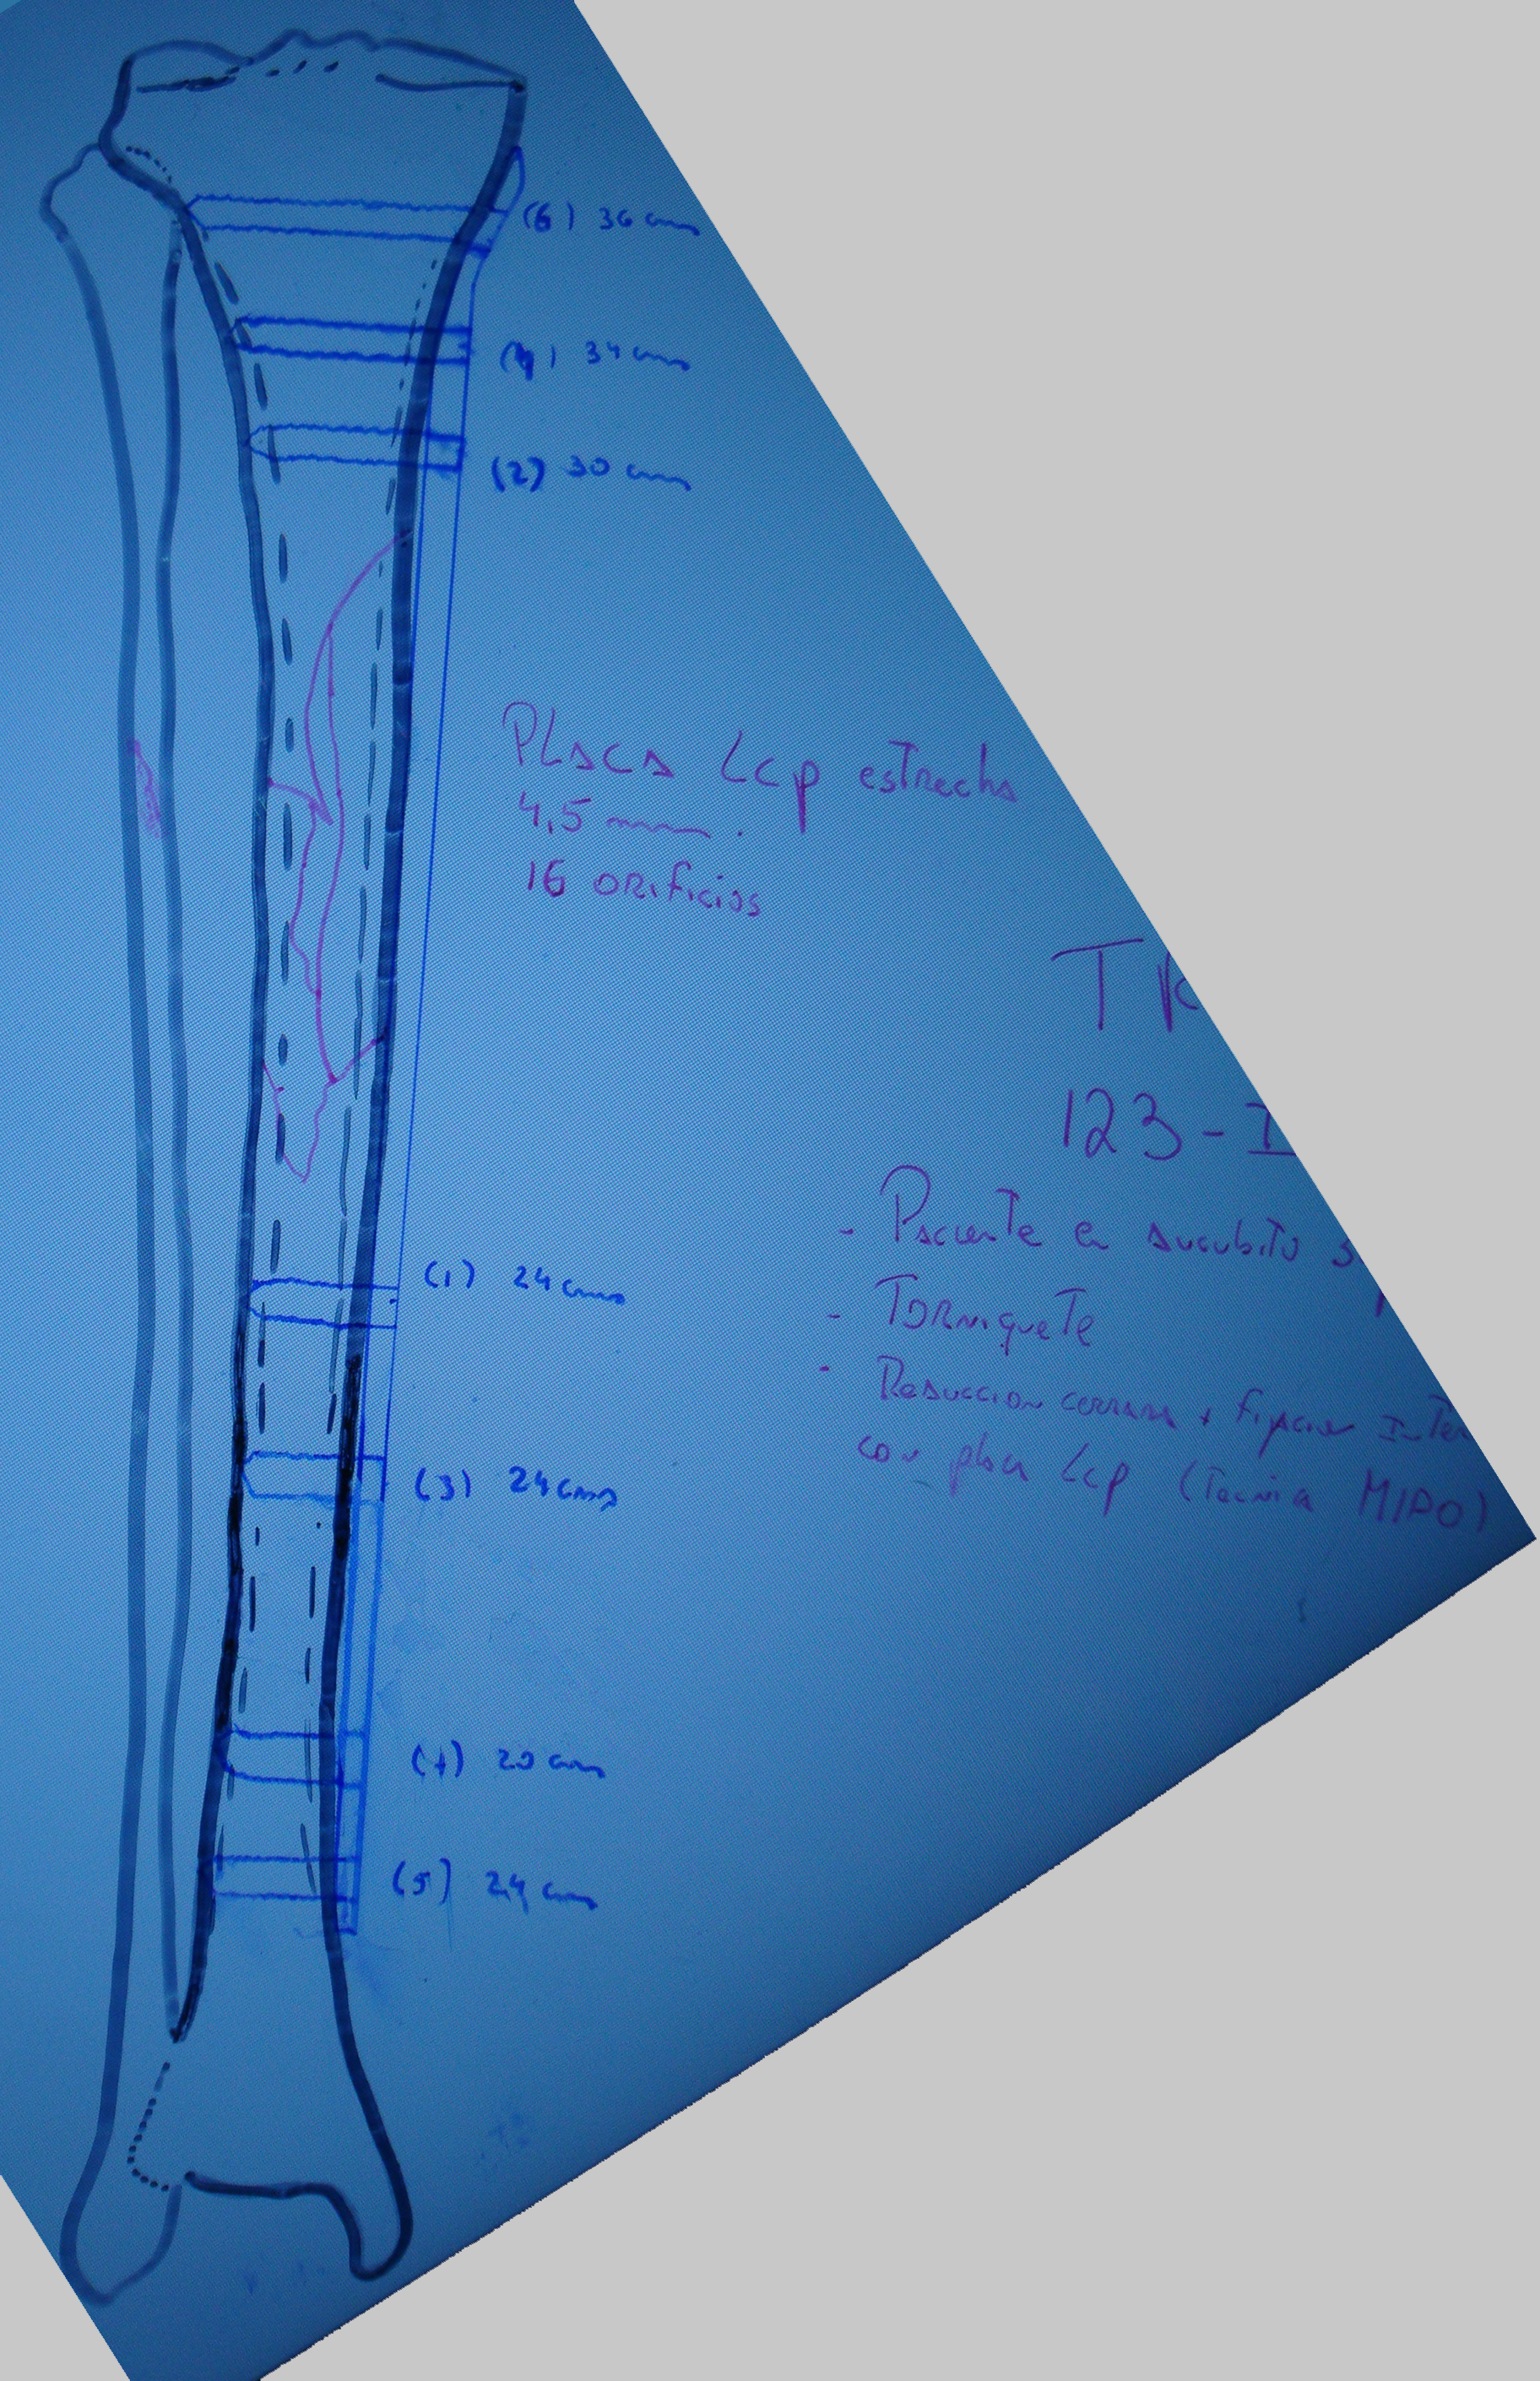
\includegraphics[width=0.40\columnwidth]{images/casoconvencional.png}} \hspace{0.10cm}
\subfigure[]{\label{fig:casoconvencional2}\includegraphics[width=0.54\columnwidth]{images/casopropuesta.png}}
  \end{center}
  \caption{Un ejemplo de planificaci\'on preoperatoria para una fractura del tipo 42C3 donde se realiz\'o la (a) planificaci\'on convencional y la (b) planificaci\'on empleando nuestra propuesta} 
  \label{fig:casoconvencional}
\end{figure}

En dicha planificaci\'on convencional se indican los fragmentos de hueso en color morado con respecto al color azul tanto del hueso como del implante y el tornillo. Se puede observar como la calidad de la imagen depende de la precisi\'on que tenga el m\'edico al momento de realizar la planificaci\'on. Por otro lado la letra escrita colocada sobre la planificaci\'on puede variar de m\'edico en m\'edico, dificultando en algunas ocasiones la lectura del mismo. Un factor a destacar es la orientaci\'on de la planificaci\'on al momento de ser realizada. N\'otese que la imagen ha sido rotada para poder ser le\'ida correctamente. El m\'edico traumat\'ologo que la realiz\'o era zurdo, por lo cual tiende a inclinar la hoja de calco para que sea m\'as c\'omodo realizar la planificaci\'on sobre ella. El mismo escenario ocurre en el caso donde el m\'edico es diestro pero la planificaci\'on es rotada en el sentido contrario a las agujas del reloj.

Al emplear el mismo caso cl\'inico de fractura mostrado anteriormente pero empleando nuestra propuesta, se obtiene un resultado como el que muestra la Figura \ref{fig:casoconvencional2}. Claramente se pueden observar las ventajas de una planificaci\'on digital contra una convencional. Es posible colocar diversos colores para indicar m\'as claramente los materiales a utilizar. Las medidas son m\'as precisas con respecto a la realidad adem\'as de quedar indicadas en un color que contraste con la placa. Adem\'as, los fragmentos de huesos son armados correctamente y se indica el proceso en una lista con instrucciones y notas para la cirug\'ia.

La planificaci\'on preoperatoria empleando nuestra propuesta permite establecer lineamientos en la realizaci\'on de este procedimiento. Esto permite tener una mayor facilidad de comprensi\'on de los estudios planificados,  disminuir los errores a nivel de medici\'on, permitir la reproducci\'on m\'ultiple y permitir corregir errores sin ocasionar repercusiones a nivel visual en el resultado.

Las im\'agenes presentadas en la Figura \ref{fig:casoconvencional} fueron tomadas con permiso de un paciente que ingres\'o al HUC con fractura producto de una ca\'ida en motocicleta. Con la planificaci\'on preoperatoria digital se pudo realizar de manera exitosa la cirug\'ia correspondiente y el paciente se pudo recuperar adecuadamente bajo los tratamientos post-operatorios que le fueron indicados por el m\'edico tratante. En la Figura \ref{fig:casopost} se observa una placa post-operatoria donde se observa el resultado despu\'es de la operaci\'on.
\begin{figure}[htb]
	\centering
		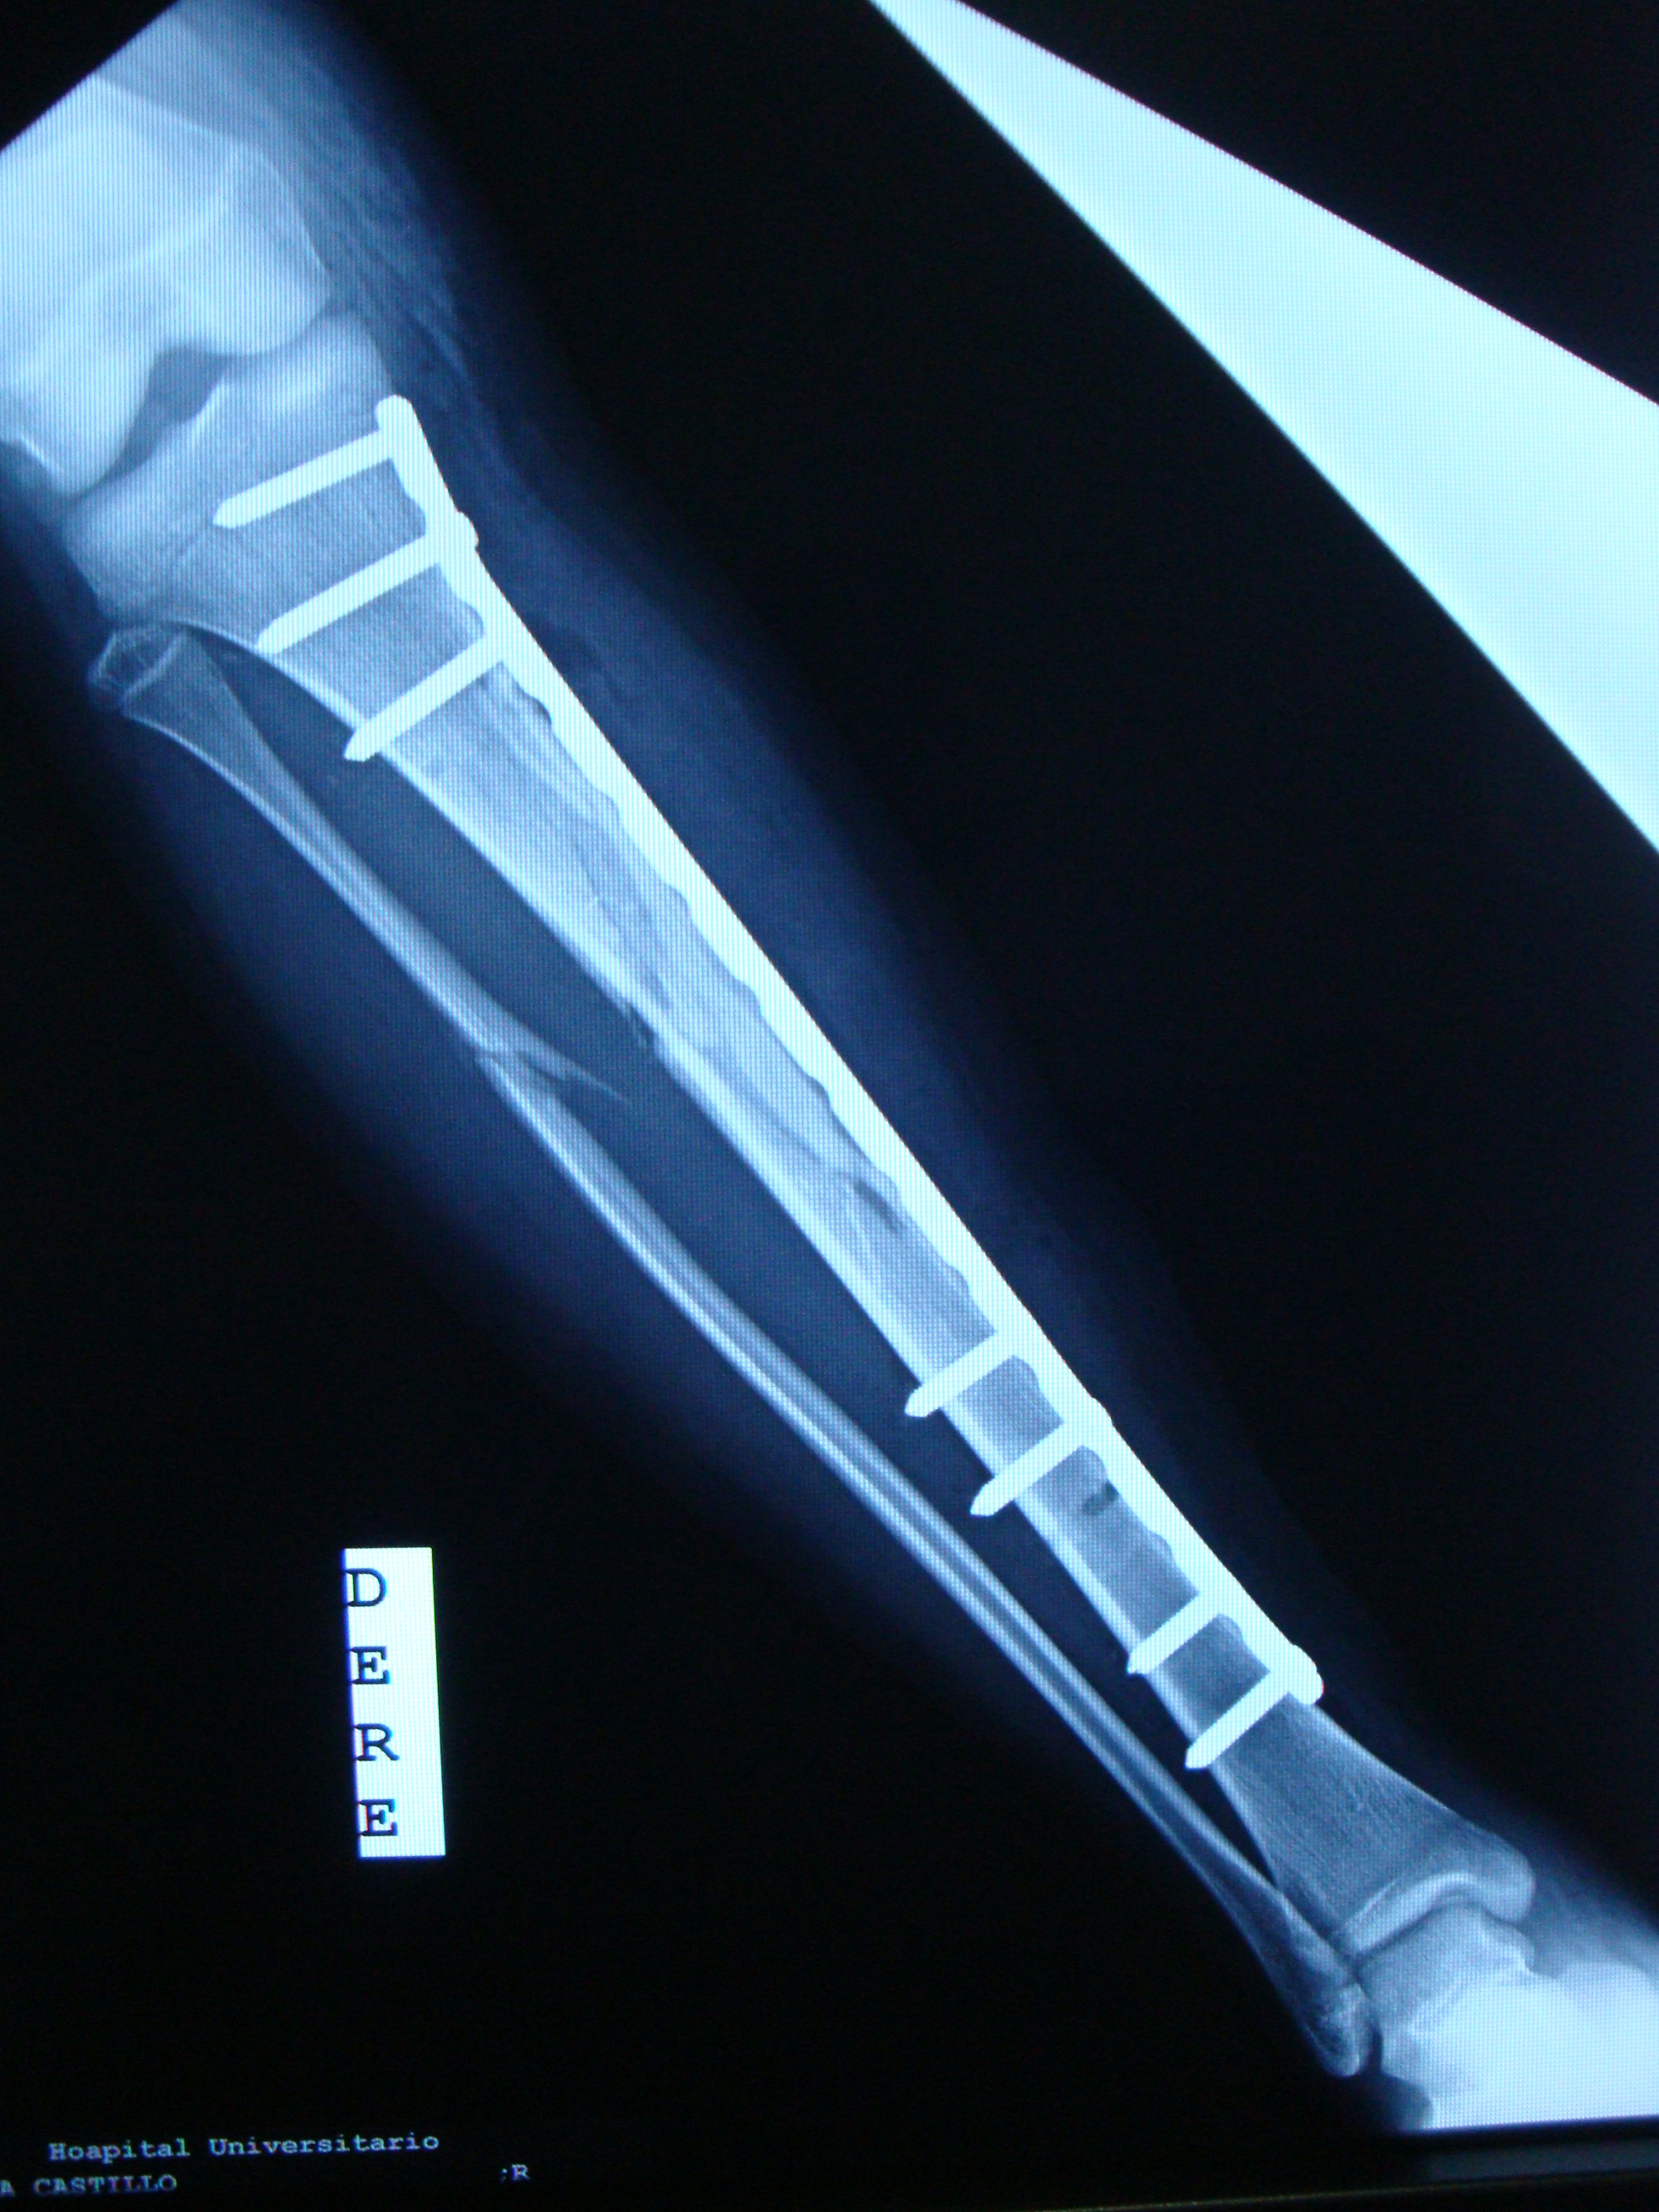
\includegraphics[width=.6\columnwidth]{images/casopost.png}
	\caption{Placa de Rayos-X realizada despu\'es de la cirug\'ia de un paciente con fractura del tipo 42C3. La placa corresponde con el mismo paciente mostrado en la Figura \ref{fig:casoconvencional}}
	\label{fig:casopost}
\end{figure}

Es importante destacar la similitud del objetivo inicial planteado al realizar la planificaci\'on preoperatoria empleando nuestra propuesta, ver Figura \ref{fig:casoconvencional2}, con el resultado obtenido despu\'es de la cirug\'ia como se muestra en la Figura \ref{fig:casopost}. De esta manera se demuestra la eficacia de la soluci\'on planteada con respecto a la soluci\'on esperada.